\documentclass[conference,10pt]{IEEEtran}
%\documentclass[conference,draft,onecolumn]{IEEEtran}
% useful packages, copy and paste from diff sources

\usepackage[english]{babel}
\usepackage[T1]{fontenc}
\usepackage{cite,url,color} % Citation numbers being automatically sorted and properly "compressed/ranged".
\usepackage{graphics,amsfonts}
\usepackage{epstopdf}
\usepackage[pdftex]{graphicx}
\usepackage[cmex10]{amsmath}
% Also, note that the amsmath package sets \interdisplaylinepenalty to 10000
% thus preventing page breaks from occurring within multiline equations. Use:
\interdisplaylinepenalty=2500
% after loading amsmath to restore such page breaks as IEEEtran.cls normally does.
\usepackage[utf8]{inputenc}
% Useful for displaying quotations
%\usepackage{csquotes}
% Compact lists
%\let\labelindent\relax
\usepackage{enumitem}
\usepackage{multirow}
%tikz figures
\usepackage{tikz}
\usetikzlibrary{automata,positioning,chains,shapes,arrows}
\usepackage{pgfplots}
\usetikzlibrary{plotmarks}
\newlength\fheight
\newlength\fwidth
\pgfplotsset{compat=newest}
\pgfplotsset{plot coordinates/math parser=false}

\usepackage{array}
% http://www.ctan.org/tex-archive/macros/latex/required/tools/
%\usepackage{mdwmath}
%\usepackage{mdwtab}
%mdwtab.sty	-- A complete ground-up rewrite of LaTeX's `tabular' and  `array' environments.  Has lots of advantages over
%		   the standard version, and over the version in `array.sty'.
% *** SUBFIGURE PACKAGES ***
%\usepackage[tight,footnotesize]{subfigure}
\usepackage{subfig}

\usepackage[top=1.5cm, bottom=2cm, right=1.6cm,left=1.6cm]{geometry}
\usepackage{indentfirst}

\usepackage{times}
% make sections titles smaller to save space
%\usepackage{sectsty}
%\sectionfont{\large}
% enable the use of 'compactitem', a smaller 'itemize'
%\usepackage{paralist}

% MP
% to split equations using dmath env
\usepackage{breqn}
% nice rules in tables
\usepackage{booktabs}
\usepackage{lipsum}


%\setlength\parindent{0pt}
\linespread{1}

% MC
\newcommand{\MC}[1]{\emph{\color{red}MC says: #1}}
\newcommand{\AZ}[1]{\emph{\color{blue}AZ says: #1}}
\newcommand{\MP}[1]{\emph{\color{green}MP says: #1}}

\usepackage{placeins}
\usepackage{dblfloatfix}

\setlength{\belowcaptionskip}{-8pt}

%%%%%%%%%%%%%%%%%%%%%%%%%%%%%%%%%%%%%%%%%%
\begin{document}
%%%%%%%%%%%%%%%%%%%%%%%%%%%%%%%%%%%%%%%%%%
\title{V2X mmWave Connectivity with Real Velocity Traces}

\author{\IEEEauthorblockN{Luca Della Libera, Jacopo Pegoraro, Andrea Rossi}
\IEEEauthorblockA{Department of Information Engineering, University of Padova -- Via Gradenigo, 6/b, 35131 Padova, Italy\\Email: {\tt\{luca.dellalibera.1, jacopo.pegoraro, andrea.rossi.26\}@studenti.unipd.it}
}}

\maketitle

\begin{abstract}
The millimeter wave (mmWave) bands offer the opportunity to exceptionally increase the data rates for fifth-generation cellular systems and support the birth of emerging automotive applications. The performance of end-to-end communications dramatically decreases when there are obstacles in the Line-Of-Sight (LOS) between a user and a mmWave base station.
This paper analyzes the performance of UDP protocol under different handover policies, in a urban automotive scenario based on real world traffic data simulation traces generated with SUMO (an open source simulator which allows traffic systems modeling) \cite{sumo} and imported in a network simulation platform like ns-3 \cite{ns3}. In a future urban scenario, important information such as the route of a vehicle from a starting point to a destination could be effectively employed to predict which base station is more suitable to ensure a better connection. The purpose of this paper is showing that these policies, combined with a prior knowledge of the scenario, can improve the throughput and/or delay of the connection.
\end{abstract}

%%%%%%%%%%%%%%%%%%%%%%%%%%%%%%%%%%%%%%%%%
\section{Introduction}\label{sec:intro}
%%%%%%%%%%%%%%%%%%%%%%%%%%%%%%%%%%%%%%%%%

In the last few years, a vast number of automotive applications were developed and many of them are already being tested on the latest generation vehicles: self-driving cars, sensors for real time object recognition and infotainment are only some examples. However, a fundamental prerequisite to effectively implement these applications is to have high data rates communication capabilities, since the required sensors and devices can produce data in the order of magnitude of hundreds of Mb/s \cite{surveh}.
The state of the art protocol for communication in a vehicular environment is the \emph{dedicated short-range communication} (DSRC), which still cannot satisfy the mentioned requirements, having a theoretical rate of 27 Mb/s \cite{surveh}. For this reason, there is growing interest in the potential of mmWave technologies, that make use of the frequency spectrum over 10 GHz, providing data rates in the order of Gb/s. These transmission capabilities can be achieved using carriers at very high frequency, therefore increasing the available bandwidth that could be exploited and consequently the capacity of the radio links. Nevertheless, there are some drawbacks of this approach that become even more significant in outdoor and vehicular situations. The most critical one is the high attenuation that mmWave signals are subjected to, since the \emph{path-loss} in a radio channel depends on the reciprocal square-root of the wavelength $\lambda$, so reducing $\lambda$ (increasing frequency) the path-loss increases, thus there is need for more mmWave base stations (known as mmWave enhanced Node Base - eNB) to avoid lack of coverage. Another problem is that, in order to prevent the just mentioned high attenuation, massive MIMO is used to convey the signal into narrow directional beams instead of the isotropic transmission used in present-day standards, so, when dealing with a fast-moving nodes scenario, as can be a vehicular one, mmWave technologies perform poorly due to blockage and bad beam aligning \cite{mmvehicle}.

To partially solve these problems in a future urban scenario with high density of mmWave base stations, we can work on optimizing the handover (HO) procedure, that is the technique used to control the switch of a User Equipment (UE) between different base stations, as it moves through the scenario. The current handover rule adopted in mmWave networks is the one inherited from the 4G-LTE standard and it is based on connecting to the base station that provides the maximum received SINR among those that are reachable. In this paper, we simulate a typical urban scenario and we test four different handover policies, beginning with the standard one and then checking whether slight modifications of it can lead to an improvement in terms of throughput and/or delay.


%%%%%%%%%%%%%%%%%%%%%%%%%%%%%%%%%%%%%%%%%%%%
\section{Related Work}\label{sec:sota}
%%%%%%%%%%%%%%%%%%%%%%%%%%%%%%%%%%%%%%%%%%%%

The interest for mmWave bands, between 30 and 300 GHz, where the available bandwidth is much wider than today's cellular networks, is growing more and more. Many researches have been conducted for analyzing challenges and opportunities that mmWave presents at different layers of the protocol stack, in order to support the massive demand for high data rates that is expected to be required in the next generation of automotive applications.
Rangan et al. \cite{mmwpac} analyze various technologies, including adaptive beamforming, multihop relaying, heterogeneous network architectures, and carrier aggregation used in the mmWave context, highlighting that, for what concerns outdoor coverage, these systems offer a capacity at least one order of magnitude higher than the current state of the art LTE networks.

Regarding highly dense or highly mobile vehicular scenarios, Giordani et al. \cite{mmvehicle} observe that vehicles are subjected to frequent handover, and obstacles can undermine a successful communication even if the automotive nodes are perfectly aligned, since mmWave cannot penetrate through solid materials. Furthermore, as stated in \cite{mmwvehcom}, beam alignment can exploit the geographical position of the UEs in order to limit the search area of the most favorable beam direction. Anyway, according to their analysis, the performance strictly depends on parameters such as number and velocity of the UEs, beam tracking periodicity and specific environment in which the vehicles are deployed.

\begin{figure*}[ht]
	\begin{center}    
		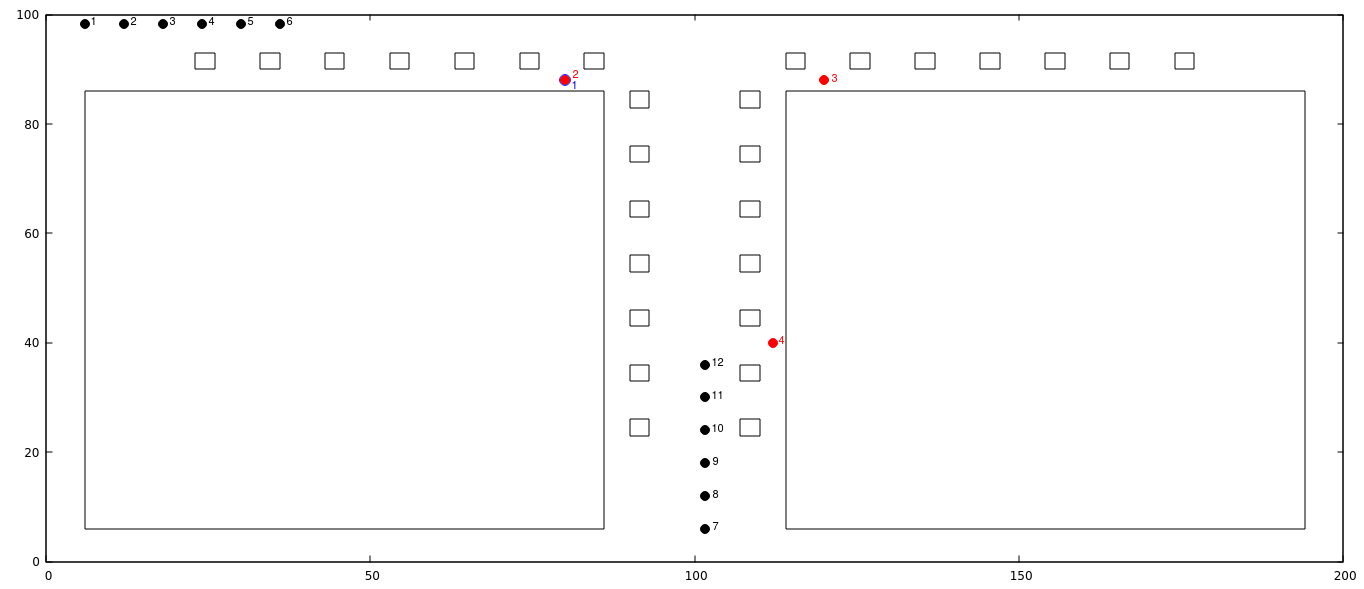
\includegraphics[width=16cm, keepaspectratio]{images/scenario.eps}
		\label{fig:scenario}
	\end{center}
	\vspace*{-6.5pt}
	\caption{The simulation scenario.}
	\vspace*{-6.5pt}
\end{figure*}

To better capture the most significant aspects of mmWave in vehicular networks, New York University and University of Padova developed an open source mmWave module for ns-3 \cite{mmwmodule}, based on LTE architecture. Mezzavilla et al. \cite{e2esim} provide some interesting code examples, showing how this module can be used to set up a simulation.

Another interesting work, proposed by Polese et al. \cite{imphand}, discusses the use of Dual-Connectivity (DC) for improving the performance of a mmWave communication. DC consists in integrating, in the same scenario, both mmWave (which has high bitrate but small area coverage) and LTE (which has low bitrate but wide area coverage) base stations that overcome each other's disadvantages: for instance, a device that experiences blockage and can no longer connect to a mmWave station, can switch to a LTE one, which is not subjected to the same blockage problems and can guarantee a lower but non-zero throughput.

None of the previously mentioned researches analyze what happens in a real world situation: for this reason, we focus on a realistic urban traffic environment and we propose alternative handover procedures, that achieve better performances in term of QoS metrics.

In the next sections, we describe the scenario and the handover policies, discussing the most relevant results of the simulations.


%%%%%%%%%%%%%%%%%%%%%%%%%%%%%%%%%%%%%%
\section{System Model}\label{sec:symo}
%%%%%%%%%%%%%%%%%%%%%%%%%%%%%%%%%%%%%%
The system model description is divided into two subsections: in the first one, we describe the simulation scenario, pointing out the most relevant configuration parameters; in the second one, we present the different policies we tested to improve QoS metrics, focusing in particular on downlink throughput and delay.


\subsection{Description of the simulation scenario}

The construction of the simulation scenario consists of two steps: the realization of the urban environment with SUMO, which generates realistic speed and position traces of the vehicles, and the usage of these traces to build the network infrastructure with ns-3.

For what concerns the first step, we opted for a trade-off between the complexity of the scenario, which is necessary to make the mmWave connectivity as challenging as it could be in a real world situation, and the amount of computational resources required to run a simulation (which can last from several hours up to few days, varying with the complexity). We reproduced a T-shaped crossroad with a traffic light in the middle (Figure 1, all distances are expressed in meters): the horizontal road has only one lane, while the vertical one has two lanes, allowing traffic in both directions. There are 12 vehicles divided into three flows, depending on the route they follow: UEs 1, 2, 4, 5 belong to the left-to-right flow, UEs 3 and 6 to the left-to-bottom flow, UEs 7, 8, 9, 10, 11, 12 to the bottom-to-right flow.
In the beginning, the traffic light is green for the bottom-to-right flow and for the left-to-bottom flow, therefore UEs 12, 11, 10, 9, 8, 7, 6 are allowed to transit (notice that UEs 4 and 5 prevent UE 3 from moving, since there is only one lane). After 45 s, the traffic light switches and all the remaining UEs rapidly reach their destinations.

Regarding the second step, the mobility traces of the vehicles were imported in ns-3, and using the mmWave module \cite{mmwmodule}, we deployed 3 base stations, in particular 2 pure mmWave eNBs (eNB 3 and 4) and 1 hybrid mmWave-LTE eNB, that acts as a link towards the Internet and makes use of the DC mechanism previously mentioned \cite{imphand}, in order to achieve a more reliable connection. Moreover, it serves as a coordinator for the handover procedure, in the sense that, after collecting information on the other eNBs SINRs with fixed time periodicity, it decides, according to some criterion, which UE connects to which eNB. In our implementation, the hybrid eNB consists of two overlapping eNBs (eNB 1 and 2), a mmWave and a LTE one, which are deployed in the same position. To make the scenario more realistic, buildings and trees were added at the sides of the roads to prevent UEs from being always in LOS condition, making connections harder to establish.

The networking side of the model was implemented using \texttt{MmWaveHelper} class of mmWave ns-3 module, which installs the mmWave physical channel and the upper layers of the protocol stack in all the devices involved in the simulation (including the X2 protocol for the communication between the LTE coordinator eNB and the other eNBs). The core network, which provides Internet connectivity to each node, was simulated through a remote host, connected to a gateway, which is in turn connected to the LTE coordintator eNB.

The channel model adopted in this scenario is \emph{3GPP UMi-StreetCanyon}, which is reliable provided that the 2D distance between an eNB and a UE is greater than 10 m and the height of a UE is greater than 1.5 m. The maximum bitrate that a single eNB can guarantee with this configuration is 3 Gbit/s. In a real world scenario, problems occur when the total throughput required by UEs exceeds eNB capacity. In order to saturate the eNBs, we ran on each UE a UDP application which demands 1054 byte packets with interarrival time of 1 $\mu$s.

All details about simulation parameters are shown in Table I. This configuration was used to test four different handover procedures, which will be presented in the next section.

\begin{table}[t]
	\begin{center}
		\begin{tabular}{ccc}
			\toprule
			
			Parameter & Value & Description  \\
			\midrule
			
			T$_{sim}$ & 60 s & Duration of the simulation \\
			T$_{phase}$  & 45 s & Duration of the traffic light red phase \\
			T$_{UDP}$ & 1 $\mu$s & Packet interarrival time \\
			D$_{SINR}$ & 25.6 ms & SINR report periodicity \\	
			V$_{max}$ &  13.8 m/s & Upper bound for random UE speed \\
			L$_{pck}$ & 1054 byte & UDP packet size \\
			d$_{UE-eNB}$ & 12 m & 2D Distance between UEs and eNBs \\		
			d$_{UE}$ & 1.5 m & Minimum gap between vehicles \\
			h$_{UE}$ & 1.6 m & Height of the UEs \\
			h$_{eNB}$ & 3 m & Height of the eNBs \\
			h$_{building}$ & 25 m & Height of the buildings \\
			h$_{tree}$ & 5 m & Height of the trees \\
			\bottomrule
		\end{tabular}
	\end{center}
	\vspace*{-2pt}
	\caption{Simulation parameters.}
    \vspace*{-6.5pt}
\end{table}

\noindent
\subsection{Handover policies}
The following four policies were tested on the simulation scenario:

\begin{enumerate}
\item \emph{DHO}: \emph{Default Handover} is the standard rule used nowadays by LTE cellular networks and has its core in the criterion used by the LTE coordinator to decide when a UE has to switch between two base stations. The procedure is summarized in the following steps \cite{imphand}:

\begin{itemize}
	\item The coordinator monitors the received SINR by a UE from all the eNBs.
	\item Whenever an eNB (target eNB) provides a SINR at least 3 dB higher than the current one, the coordinator keeps track of the difference between the two SINRs for a time equal to TTT (Time-To-Trigger) seconds.
	\item If the target eNB keeps providing more than 3 dB higher SINR for all the duration of TTT, the coordinator makes the UE switch to the target eNB.
\end{itemize}
Figure 2 shows an example of how switching is performed in DHO policy (eNB 1 SINR is not shown, because the SINRs of mmWave eNBs are always high enough to prevent UEs from switching to LTE). In \cite{imphand}, the authors analyze two different ways to choose the TTT value: one is to keep it fixed at, for example, f$_{TTT}$ = 150 ms; the other is to have a \emph{dynamic} threshold that increases as the difference $\Delta$ between the current eNB SINR and the target eNB SINR decreases.

\begin{figure}[!t]
	\vspace*{-7.0pt}
	\begin{center}    
		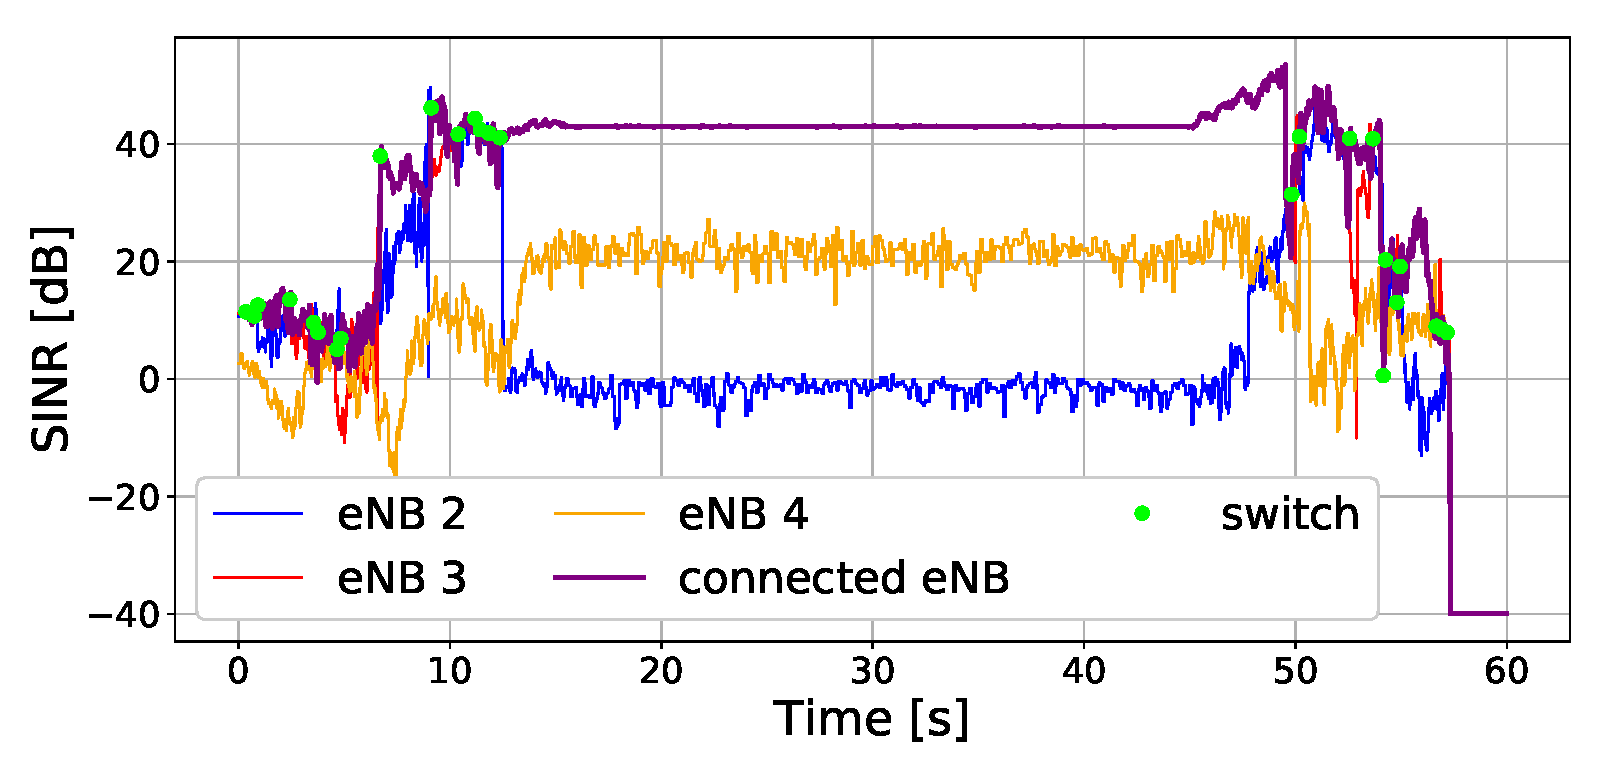
\includegraphics[width=8.8cm, keepaspectratio]{images/ue4_switch_dho.eps}
		\vspace*{-0pt}
	\end{center}
	
		\caption{DHO, UE 4.}
		\vspace*{-10pt}
\end{figure}

\item \emph{MHO100}:
\emph{Modified Handover 100} relies on a fixed threshold value SINR* = 100 (in linear scale) and performs the following steps:

\begin{itemize}
	\item The coordinator keeps track of the maximum SINR received for each UE.
	\item If there are SINRs from one or more eNBs that are close enough to the maximum one, in the sense that the difference between the two is lower than SINR*, the coordinator triggers the handover towards the eNB that has the lowest number of connected UEs.
	\item If, according to the previous rule, none of the eNBs are a good candidate for the handover, the UE connects to the maximum SINR eNB. If there are many candidate eNBs with the same number of connected UEs, the one with maximum SINR is chosen.
\end{itemize}

The goal of this method is considering that both the throughput and the delay can strongly depend on the level of congestion of the eNBs, due to the excessive number of connected vehicles. SINR is indeed a good metric of path-loss, blockage and quality of the channel, but it does not capture the number of users that the eNB is currently handling.

\item \emph{MHOM}:
\emph{Modified Handover Mean} follows the same procedure of MHO100, with a dynamic threshold value, computed as the arithmetic mean of the SINRs received from the three mmWave eNBs. In this way, SINR* is able to adapt to many circumstances, considering the fact that, in such a fluid scenario, SINR usually varies exponentially from 1 dB up to 40 dB. Furthermore, since SINR* is a function of the SINR of all eNBs, it can handle situations in which the three SINRs are very different from each other.

\begin{figure*}[!t]
	\begin{center}
	\begin{minipage}{.245\textwidth}
		\centering
		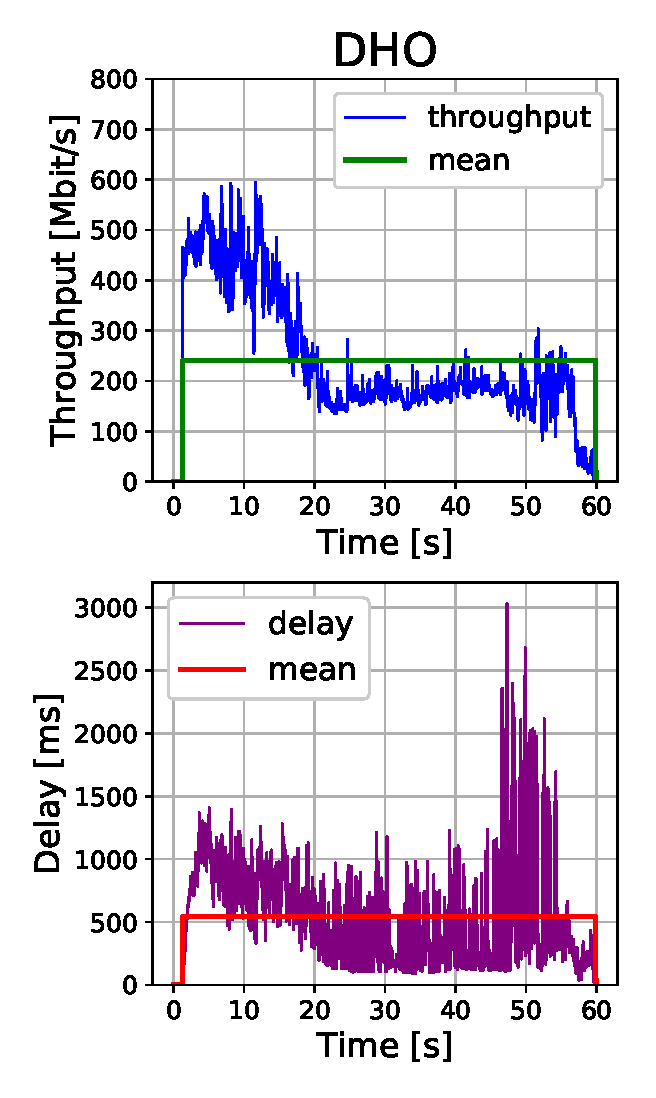
\includegraphics[width=\linewidth, keepaspectratio]{images/results_dho.eps}
		\label{fig:test1}
	\end{minipage}%
	\begin{minipage}{.245\textwidth}
		\centering
		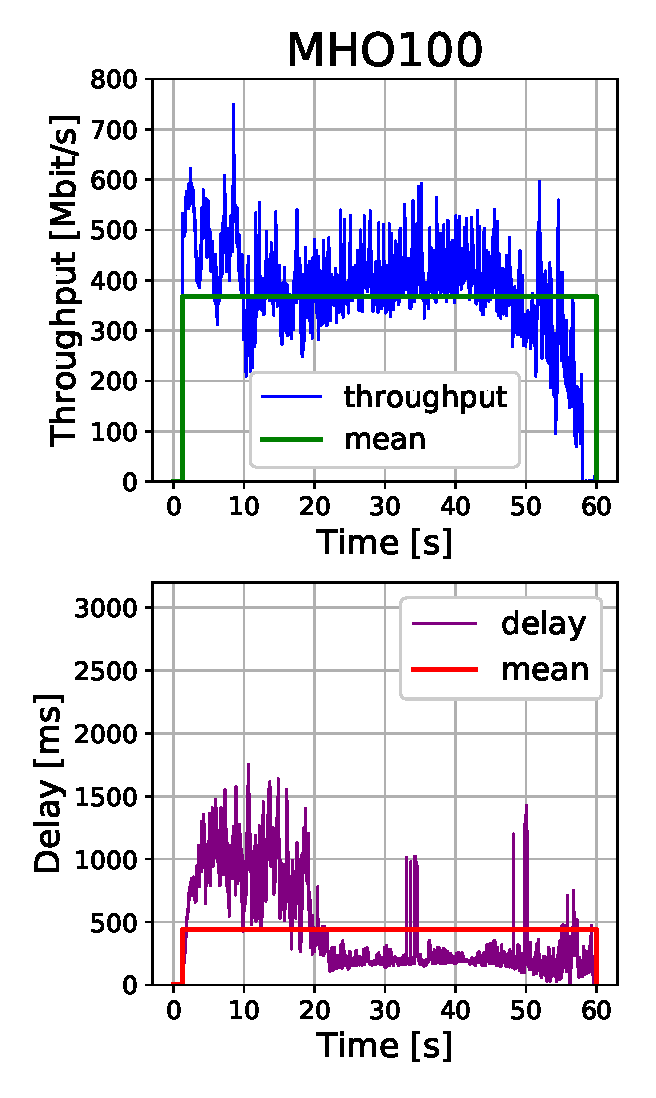
\includegraphics[width=\linewidth, keepaspectratio]{images/results_mho_100.eps}
		\label{fig:test2}
	\end{minipage}
	\begin{minipage}{.245\textwidth}
		\centering
		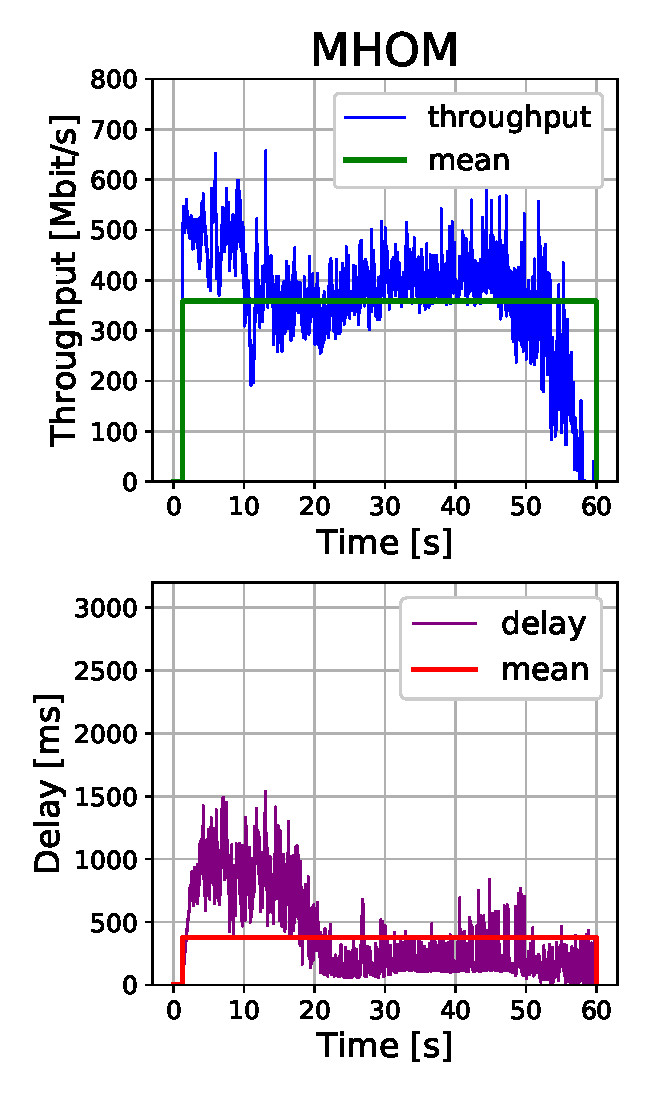
\includegraphics[width=\linewidth, keepaspectratio]{images/results_mho_mean.eps}
		\label{fig:test3}
	\end{minipage}
	\begin{minipage}{.245\textwidth}
		\centering
		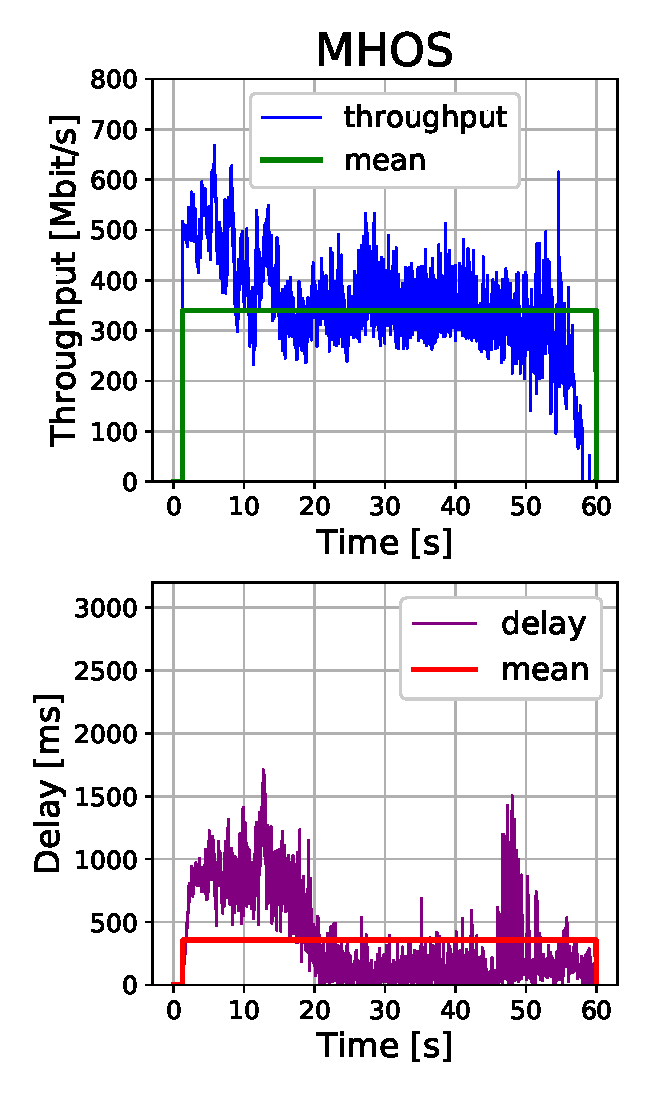
\includegraphics[width=\linewidth, keepaspectratio]{images/results_mho_shannon.eps}
		\label{fig:test4}
	\end{minipage}
	\end{center}
	\vspace*{-14pt}
	\caption{Comparison among four handover policies.}
	\vspace*{-6.0pt}
\end{figure*}

\item \emph{MHOS}:
\emph{Modified Handover Shannon} is based on a different approach. The goal is maximizing the capacity of the channel used by the UEs, taking into account the congestion by means of Shannon formula for channel capacity. The channel capacity offered by a base station $i$ can be approximately expressed as:
 $$
 C_i=\frac{1}{N_i} B \log_2(1+SINR_i)
 $$
\noindent where $N_i$ is the number of UEs connected to the $i$-th eNB, $B$ is the channel bandwidth and $SINR_i$ is the SINR (in linear scale) received from the base station $i$.
The proposed policy performs the following steps:

\begin{itemize}
	\item The UE is initially connected to the eNB $i$.
	\item Let $j$ be the index of the target eNB, which provides a SINR equal to $SINR_j$ to the current user and has $N_j$ UEs connected. The coordinator triggers the handover towards the eNB $j$ if it offers a higher channel capacity than eNB $i$. In formulas:
	$$
	\frac{1}{N_i} \log_2(1+SINR_i) < \frac{1}{N_j+1} \log_2(1+SINR_j)
	$$ 
\end{itemize}
\noindent Notice that the bandwidth can be simplified from the expression (since it is the same) and that $N_j$ has to be incremented by one because, if the handover is performed, the target eNB will have one more UE to handle.
\end{enumerate}

It is worth considering that the three modified policies take into account, even though in an indirect way, the route followed by a UE, because at every instant the number of UEs connected to a certain eNB depends on how the scenario evolved in the past. For instance, with DHO policy, the UEs waiting at the traffic light will connect to the closest eNB. As the vehicles continue to enqueue, the eNB will rapidly reach a high level of congestion, becoming unable to satisfy the requests of all UEs. On the contrary, with a MHO policy, there are chances that the UEs closer to the crossroad, receiving a lower but still good signal from another eNB, which is not saturated (because the vehicles coming from the other direction are moving, since the traffic light is green), will switch to this eNB, freeing up resources for the other UEs. In such a situation, MHO is able to 'detect' the presence of a traffic light, and act consequently. These policies are indeed a mixture between the current memoryless handover procedure, which does not consider the level of congestion, and the smart AI-based procedures of the future, which will be able to distribute the traffic depending on the route followed by a UE. However, these advanced techniques will be appliable when self-driving interconnected vehicles, that share information among each other, will become a common standard.

%%%%%%%%%%%%%%%%%%%%%%%%%%%%%%%%%%%%%%%%%%%%%%%
\section{Results}\label{sec:res}
%%%%%%%%%%%%%%%%%%%%%%%%%%%%%%%%%%%%%%%%%%%%%%%

In this section, we explain the mathematical approach we used to analyze the data and we compare DHO with the other three policies previously described.
First of all, it is important to point out that, due to computational power constraints, the scenario is deterministically fixed, while in a real world environment there are thousands of possible situations, thus the validity of our results applies only to this specific case. To partially solve this problem, in order to extend the generality of our analysis, we decided to include randomness in the physical channel. Therefore, the data we collected are the result of twenty simulations, five for each of the four policies we had to test.

The QoS metrics we consider are the downlink throughput and the delay at PDCP, a common transport layer protocol used in vehicular communications. The throughput of a single simulation was computed by sampling the received packets every 25.6 ms (the same interval of SINR report periodicity), summing the total amount of bits received in this interval and dividing by its duration, as described in \cite{imphand}. A similar approach was used to calculate the delay, with the only difference that, instead of summing the delay of each packet, we computed the mean delay of the packets received in the same interval (since delay is not additive). Finally, we computed the statistical mean of throughput and delay over the five collected traces. We noticed that the results were not uniform for all UEs: some of them experienced an improvement, some other a worsening of throughput and delay. In order to evaluate the global performance of the policy, we computed the weighted mean of instantaneous throughput and delay over the 12 UEs (assigning as a weight the percentual of time that each UE spends in the scenario before quitting the simulation), and then calculated the corresponding time average value.

\begin{table}[t]
	\vspace*{9pt}
	\begin{center}
		\begin{tabular}{cccc}
			\toprule
			HO policy & Throughput [Mbit/s] & Delay [ms] & Number of HO \\
			\midrule
			DHO & 241 & 542 & 190 \\
			MHO100 & 368 & 439 & 218 \\
			MHOM & 359 & 376 & 204 \\
			MHOS & 340 & 358 & 249 \\			
			\bottomrule
		\end{tabular}
	\end{center}
		\caption{HO policies results.}
	\vspace*{-6.5pt}
\end{table}
Table II reports the final results of the four policies. As shown by the plots in Figure 3, each method achieves significant improvements of the two considered metrics. In particular, among the proposed policies, MHO100 performs better in terms of throughput, obtaining a 52.7\% improvement in comparison with DHO. For what concerns delay, MHOS achieves the best result with a 33\% reduction in comparison with DHO. MHOM represents a trade-off between the other two, improving considerably both the throughput (48.9\%) and the delay (30.6\%), but not as much as MHO100 and MHOS respectively. The choice of the policy depends on the requirements the system needs to satisfy: if the priority is a high throughput, MHO100; if the priority is a low delay, MHOS; otherwise, if both a high throughput and a low delay are required, MHOM. Anyway, if we had to consider the general validity of these policies, we would discourage the adoption of MHO100 for one main reason: it uses a fixed threshold value. In general, a fixed strategy is not a good choice because it works well only in few situations. Therefore, since we tested just one scenario, MHO100 gives less performance guarantees than an adaptative strategy such as MHOM.

It is worth pointing out that the proposed procedures improve the metrics especially starting from 20 - 25 s. That is the interval of time when the first seven vehicles (six belonging to the bottom-to-right flow, one to the left-to-bottom flow) disconnect after reaching their destinations, while the other five (four belonging to the left-to-right flow, one to the left-to-bottom flow) are enqueued at the traffic light. This is exactly the expected behaviour: DHO connects the waiting UEs to the closest eNB, increasing the level of congestion, while our policies tend to split the UEs among the further (but still close enough to provide a good SINR), less congested eNBs.

\begin{figure}[h]
	\vspace*{-6pt}
	\begin{center}    
		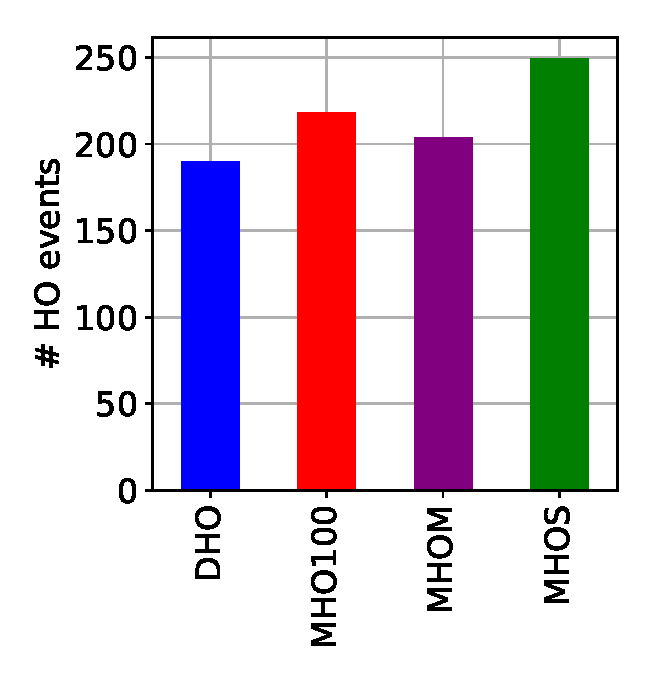
\includegraphics[width=5cm, keepaspectratio]{images/ho_events.eps}
	\end{center}
	\vspace*{-10pt}
	\caption{Number of HO events.}
	\vspace*{3pt}
\end{figure}

Finally, in Figure 4, we plot the average number of handover events. As expected, we notice that this number is higher when considering the MHO policies. The reason is that, since these procedures take into account not only the SINR, but also the number of connected UEs, they are more flexible in comparison with DHO. Therefore, a UE has better chances to switch its current eNB and to adapt to the channel dynamics in a more responsive way. In particular, we observe that MHO100 and MHOM are the closest to DHO in terms of number of HO, because their threshold values are usually quite small, and if we let SINR* tend to zero, we obtain exactly DHO. Since MHOM has the lowest number of HO events among the proposed policies and still performs globally better (considering both the throughput and the delay), we conclude that MHOM triggers handover in a more selective and accurate way, in comparison with MHO100 and MHOS.

%%%%%%%%%%%%%%%%%%%%%%%%%%%%%%%%%%%
\section{Conclusions}\label{sec:conclusion}
%%%%%%%%%%%%%%%%%%%%%%%%%%%%%%%%%%%

In a real world automotive scenario, the large number of UEs connected to the same eNB can easily lead to congestion problems, especially in high traffic areas like crossroads and roundabouts. In this paper, we proposed three different handover policies, in order to improve the throughput and the delay perceived by the UEs. Running several simulations on a simple but realistic urban environment, we showed that the standard handover procedure can be improved significantly by considering the number of UEs connected to each eNB. This approach is indeed a first step towards more complex techniques based on the knowledge of the route followed by each UE, assuming that, in the next future, this kind of information will be more and more accessible due to GPS real time tracks sharing in a self-driving vehicles context.

Future developments of this work include, on one hand, the increasing of both complexity and randomness of the scenario, with the possibility to simulate the presence of pedestrians that suddenly cause blockage; on the other hand the implementation of more advanced handover policies, which rely on vehicles movement prediction.


\addtocontents{toc}{Bibliografia}
\begin{thebibliography}{15}
	
	\bibitem{surveh}
	V. Va, T. Shimizu, G. Bansal, R. W. Wealth Jr et al.,
	\emph{Millimeter Wave Vehicular Communications: A Survey}. 
	Foundations and Trends in Networking, vol. 10, no. 1, 2016.
	
	\bibitem{mmvehicle}
	M. Giordani, A. Zanella, M. Zorzi,
	\emph{Millimeter Wave Communication in Vehicuar Networks: Challenges and Opportunities}. 
	IEEE 6th International Conference on Modern Circuits and Systems Technologies, 2017.
	
	\bibitem{imphand}
	M. Polese, M. Giordani, M. Mezzavilla, S. Rangan, M. Zorzi,
	\emph{Improved Handover Through Dual Connectivity in 5G mmWave Mobile Networks}. 
	IEEE Journal on Selected Areas in Communications, vol. 35, no. 9, pp. 2069-2084, 2017.
	
	\bibitem{e2esim}
	M. Mezzavilla, M. Zhang, M. Polese, R. Ford, S. Dutta, S. Rangan, M. Zorzi,
	\emph{End-to-End Simulation of 5G mmWave Networks}. 
	arXiv preprint, 2017.
	
	\bibitem{mmwwicom}
	T. S. Rapparport, R. W: Heath Jr, R. C. Daniels, J.N. Murdock,
	\emph{Millimeter Wave Wireless Communications}.
	Prentice Hall, 2015.
	
	\bibitem{mmwcomsy}
	K. C. Huang, P. Rapajic, Z. Wang,
	\emph{Millimeter Wave Communication Systems}.
	Wiley, 2011.
	
	\bibitem{mmwpac}
	S. Rangan, T. S. Rappaport, E. Erkip,
	\emph{Millimeter-Wave Cellular Wireless Networks: Potentials and Challenges}.
	Proceedings of the IEEE, vol. 102, no. 3, March 2014.
	
	\bibitem{mmwvehcom}
	J. Choi, V. Va, N. Gonz\'{a}lez-Prelcic, R. Daniels, C. R. Bath, and R. W. Heath Jr.,
	\emph{Millimeter-Wave Vehicular Communication to Support Massive Automotive Sensing}.
	IEEE Communications Magazine, vol. 54, no. 12, December 2016.
	
	\bibitem{sumo}
	D. Krajzewicz, J. Erdmann, M. Behrisch, and L. Bieker, \emph{Recent Development and Applications of SUMO - Simulation of Urban MObility}.
	International Journal On Advances in Systems and Measurements, 5 (3\&4):128-138, December 2012.
	Available at: \texttt{http://sumo.dlr.de/index.html}.
	
	\bibitem{ns3}
	ns-3 Consortium, “What is ns-3”. Available at:\\ \texttt{https://www.nsnam.org/overview/what-is-ns-3/}.

	\bibitem{mmwmodule}
	NYU WIRELESS, University of Padova, “ns-3 module for
	simulating mmwave-based cellular systems”. Available at:\\
	\texttt{https://github.com/nyuwireless-unipd/ns3-mmwave}.
	
\end{thebibliography}

\end{document}
